%%%%%%%%%%%%%%%%%%%%%%%%%%%%%%%%%%%%%%%%%%%%%%%%%%%%%%%%%%%%%%%%%%%%%%%%%%%%%%
%
%  Main text for ``sandwich'' manuscript
%
%  Process with ``pdflatex CholColloids.tex''
%
%  The supporting material text is support.tex
%
%%%%%%%%%%%%%%%%%%%%%%%%%%%%%%%%%%%%%%%%%%%%%%%%%%%%%%%%%%%%%%%%%%%%%%%%%%%%%%

\documentclass[12pt]{article}

\usepackage{graphicx,color}

\begin{document}

\title{Self-assembly of colloid-cholesteric composites: A route to switchable optical materials}
\author{K. Stratford$^{*}$, O. Henrich$^{*}$, J.~S. Lintuvuori$^{*}$,\\
M. E. Cates, D. Marenduzzo \\ 
{\small SUPA, School of Physics and Astronomy, Edinburgh University,} \\
\small{Edinburgh, EJ9 3JZ, UK}\\
\small{$^{*}$ equally contributed to this work}}
\date{}

\maketitle

{\bf Colloidal particles dispersed in liquid crystals can form new materials with tunable elastic and electro-optic properties~\cite{stark}. In a host comprising  a periodic `blue phase' chiral liquid crystal~\cite{mermin}, the particles should template into colloidal crystals \cite{miha} with potential uses in photonics, metamaterials, and transformational optics~\cite{lavrentovich}. 
Here we show by computer simulation that colloid/cholesteric mixtures can give rise to a much wider range of soft-solid composites than previously anticipated. These include regular crystals, glasses, percolating gels, isolated clusters, twisted rings and undulating colloidal ropes. The final structure can be tuned through the particle concentration, and by varying the surface interactions of the cholesteric host with both the colloids and any confining walls. 
Remarkably, we find that many of these new materials are metastable: two or more structures can arise under identical thermodynamic conditions. The observed structure depends not only on the formulation protocol,
but also on the history of an applied electric field.  
This new class of soft materials should thus be relevant to the design of switchable, multistable devices for optical technologies including, for example, e-paper~\cite{epaper}.}

When spherical colloidal particles are mixed into a nematic liquid crystal, 
they disrupt the orientational order in the fluid and create defects (disclination lines) in the nematic close to their surfaces. To minimize the free energy cost, it is generally advantageous for defects to be shared:
therefore the colloidal particles have a generic tendency to aggregate. Such aggregates may further 
self-assemble into lines~\cite{wiresmiha}, 2D crystals~\cite{zumer}, 
planar structures~\cite{tanaka}, or 3D amorphous glasses~\cite{tiffany}.
Besides being of fundamental interest to materials science, these
structures have tunable elastic and optical properties~\cite{stark}. Hence 
they offer exciting prospects for applications as biosensors~\cite{abbott}, or
as new-generation devices~\cite{colloiddevice,electrophoresis}.

But one may also choose to disperse colloidal particles in a cholesteric, 
rather than nematic, liquid crystal. The molecules making up this material are
chiral, and this causes their average orientation (described by a director field) to rotate in space in
a helical fashion, rather than remain uniform as in nematics. 
This typically creates a 1-dimensional periodic structure, called the cholesteric phase, whose wavelength 
is the pitch, $p$. The periodicity can however become fully three dimensional in the so-called blue phases (BPs)~\cite{mermin}. BPs arise because the director field can twist around more than one direction at once (see 
the cartoon in Fig. S1). Such double twist 
regions (generally cylinders: DTCs) are energetically favoured at high enough molecular chirality, but
lead to geometric frustration because it is impossible to tile the whole 3D
space with DTCs without also introducing disclination lines: singular topological defects on which the director field is undefined. In blue phases these disclination lines themselves either form a 3D periodic regular lattice (in so called BPI and BPII), or remain disordered (BPIII)~\cite{bp3}. 
%
BPs are stabilised by the tendency of chiral molecules to twist, but destabilised by the cost of forming topological defects (which locally diminish the molecular alignment). In conventional cholesteric materials~\cite{mermin} this balance is only achievable in a narrow temperature range of a few degrees, around the onset of liquid crystalline ordering. However, recent advances in formulation have widened this stability range enormously (up to 250K) paving the way to
applications of BPs in display devices~\cite{kikuchi,bplasers,coleswidetrange,bpdevice,coles}.

Besides being remarkable materials in themselves, BPs offer significant promise as hosts for dispersing colloidal particles. Because BPs contain a disclination network even in the absence of
particles, they can potentially template colloidal self-assembly. 
This was proved recently by simulations of BP-dispersed nanoparticles which interact only weakly with the molecules of a BP (to give a so-called `weak anchoring' regime)~\cite{miha}. Such particles are attracted to the disclination network in BPs: by covering up the defect cores, the high elastic energy cost of those regions is avoided. The pre-existing order of the defect network then templates particles into a regular colloidal crystal of the same periodicity. 
Because this structure has a wavelength in the visible range, 
the resulting material should inherit (and likely enhance) the incomplete photonic bandgap of the parent blue phase, as exploited for instance in laser devices~\cite{bplasers}; for related possibilities see \cite{lavrentovich}.

A second compelling reason to study colloid-BP composites is that, even without particles, BPs can show several competing metastable free energy minima,
corresponding to different topologies of the defect network~\cite{adriano}, with a strong dependence on applied electric or magnetic fields~\cite{henrichfield}.
% 
Adding particles is likely to further enrich the free energy landscape, creating composites that might be promising candidates for bistable or multistable devices, in which energy is needed only to switch optical properties and not to maintain them. (This is the e-paper paradigm~\cite{epaper}, and can lead to huge energy savings.)
To explore such metastability, and switching strategies between states, we require multi-unit-cell, time-dependent simulations. These go beyond previous studies of colloid-BP composites~\cite{miha} but follow comparable simulations of pure BPs~\cite{bp3,henrichfield,domaingrowth}, and isolated and dimeric colloids in cholesterics~\cite{juho1,juho2}. Our methodology and simulation parameters are summarized in the Supporting Information.

We show in Fig.~1 A-D the final state structures of four simulations in which we first equilibrated a stable BPI disclination network in bulk (with periodic boundary conditions) and then dispersed colloidal particles within it. Among dimensionless control parameters are the colloid volume fraction $\phi$  ($\phi = 1\%$ or $5\%$); the ratio $r = R/\lambda$ of particle radius to the BP lattice parameter $\lambda$ (here $r\simeq 0.14$) and the ratio $w = WR/K$ where $W$ is the anchoring strength of the cholesteric at the particle surface, and $K$ is the elastic constant of the liquid crystal (defined such that $W>0$ gives preferential perpendicular orientation of the director field at the particle surface). For the latter we choose $w = 0.23, 2.3$ which are within typical experimental range~\cite{tiffany}. This parameter can be viewed as the ratio of the anchoring energy, $WR^2$, to the elastic energy scale for distortion $KR$. 

For a single colloidal particle in a nematic fluid, $w$ controls the formation of a local topological defect at the particle surface~\cite{stark}, with weak distortion of the nearby fluid at small $w$. In the colloid-BP system, $w$ also plays a determining role in the final composite structure. When $w$ is small (Fig.~ 1A,B), the attraction of particles to the disclination lattice causes
 the lattice to become covered by particles, with little disruption of its
 long-range order. Thus a templated colloidal crystal is created, as first reported in~\cite{miha}. Interestingly, the weak but finite anchoring apparently creates an elastic force between the colloids which leads to very slow dynamics (Fig. S4) and the formation of small colloidal lines within disclinations, especially for dilute samples (Fig. 1A). It seems likely that polymer-stabilised  blue phases~\cite{kikuchi} work by a similar principle to this small $w$ case, with a weak segregation of monomers towards the defect regions.

For large $w$ (Fig.~1C,D), the picture changes dramatically.
Each colloidal particle now disrupts significantly the order of the nearby fluid, with defect formation close to its surface~\cite{stark}. The resulting strong disruption of local liquid crystalline order around each particle leads now to 
a strong interparticle attraction. This restructures the disclination
network completely, destroying the long range order of
the original BPI topology. Most notably, particle aggregation favours
the formation of defect junctions, where four disclinations meet. This structural motif is present in the unit cell of BPII rather than BPI (and also seen in the amorphous BPIII~\cite{bp3}). The particle clusters are disjoint at low volume fractions ($\phi\simeq 1\%$) but they interact elastically via the connecting disclinations. At larger $\phi$, the aggregates join up to form a percolating colloidal cluster which essentially templates the disclinations rather than vice versa. 

All the structures in Fig.~1A-D should be soft solids, of nonzero elastic 
modulus $G$ at low frequency. This contrasts with pure BPs, where
$G=0$ as the fluid can flow with a finite
viscosity via permeation of molecules through a fixed defect lattice~\cite{permeation1,permeation2}. We expect the
structures in Fig.~1A-C to be only weak gels, as here the 
defect network percolates but particle contacts do not. This is broadly similar to the cholesteric-nanoparticle gel reported
in~\cite{lubensky} (with $G<1$ Pa). In contrast, the colloidal gel
structure in Fig.~1D should be much more resistant mechanically, 
due to the formation of a thick percolating particle network. The 
structure is now akin to that of the self-quenched glass found in 
colloid-nematic composites~\cite{tiffany} at much higher volume 
fraction (over 20\% as opposed to below 5\% here), for which $G\sim 10^3$ Pa.

A more practical protocol for including particles in a BPI phase is to disperse the particles in an isotropic phase, and then quenching this into the temperature range where BPI is stable. Here we know that, without particles, the kinetics can favour disordered (BPIII-like) intermediates which may be long lived or even metastable~\cite{domaingrowth}. Fig.~1E-H shows outcomes of such a quench protocol with the same parameter sets as in Fig.~1A-D. For small $w$, the particles again decorate the disclination lines, but are this time templated onto an amorphous network rather than an ordered one.
Increasing the volume fraction (Fig.~1F) leads to a more even coverage with
a better defined particle spacing. 
For large $w$, on the other hand, strong interparticle forces again dictate
the self-assembly. At low concentrations, discrete particle clusters decorate an amorphous defect lattice (Fig.~1G) whereas at higher $\phi$ a percolating network of colloid strands (the gel in Fig.~1H) is again seen. 
The structures in Fig. 1A-H have been followed for $\sim$20 ms 
(see Fig. S4); they correspond to either very slowly evolving states or 
deep metastable minima (elastic interactions are of
order $KR$ and dwarf thermal motion, see
Fig. S4 and Ref.~\cite{stark,lavrentovich}).

In display devices and other optical applications, it is typical for liquid crystals to be strongly confined (and subject to strong boundary effects), in contrast to the bulk geometries considered above. We therefore next describe how colloidal suspensions self assemble in thin sandwiches (thickness $h = 1.75 \lambda$), whose confining walls can favour either tangential (planar degenerate) or normal (homeotropic) orientation of the director field. For simplicity we here impose one or the other as a strict boundary condition.

Fig.~2A-D shows the case of normal wall anchoring on varying $\phi$ and $w$. We quench from the isotropic to the ordered phase as was done in Fig.~1E-H, and again find a metastable, amorphous disclination network (see Supporting Information). The resulting colloid-cholesteric composites are somewhat similar to those seen in the bulk: for small $w$ the particles are templated by the network (Fig.~2A,B), whereas for large $w$ we observe isolated clusters (Fig.~2C) and percolated colloidal gels (Fig.~2D), for $\phi = 1\%$ and $4\%$ respectively. There are, however, significant effects of the confining walls.
First, the normal anchoring at the wall recruits particles there,  giving (for the chosen $h$) a density enhancement of the colloids at both walls and also in the midplane (see side-views in Fig.~2A-D). Second, the clusters formed at large $w$ are themselves anisotropic with an oblate habit. These clusters
are similar to those reported experimentally for large colloids in a
cholesteric (but non-BP) host~\cite{niek}.
 
Fig.~2E-H shows comparable simulations for planar wall anchoring. 
Without colloids, planar anchoring results in a regular cholesteric helix,
with axis perpendicular to the boundary walls. 
This twisted texture develops via a set of defect loops,
which shrink and disappear to leave a defect-free sample. However,
dispersing particles with small $w$ arrests the loop shrinking process,
stabilising twisted rings (Fig.~2E) at small $\phi$, and more complicated 
double-stranded structures at larger $\phi$ (Fig.~2F).
For larger $w$, we observe thick colloidal ``ropes" about 5 colloids across
(Fig.~2E,H). These ropes undulate to follow the chiral structure of the 
underlying fluid. On increasing the density they develop branch points and finally again approach a percolating gel morphology. Note that planar wall anchoring is incompatible with the normal anchoring on the colloids (for $w>0$), which are thus repelled from both walls (see the side views in Fig.~2E-H).

An interesting question, relevant for applications to devices, is whether 
these structures can be modified, or switched, with electric fields.
Fig.~3 addresses this question, starting from amorphous Blue Phase III,
this time at a higher chirality. Dispersing colloids in this networks
results in the particle occupying the available nodes, where the order
parameter is low (Fig.~3A). Applying a high enough field along the $z$ 
direction leads to a switching to a new phase, where colloidal arrays fit 
within a network with distorted hexagonal cells (Fig.~3B). Remarkably, upon 
field removal this honeycomb structure does not find its way back to the 
configuration before switching on the field, but gets stuck into a metastable 
structure (Fig. S7), with residual anisotropy along the field switching 
direction.
The resulting multistability is indeed a prerequisite for new generation 
switchable electrooptic devices for use in energy-saving electronics-free
appliances, smart glass, and e-paper to cite just a few examples.

%FIELD SWITCHING PARA HERE
\if{The existence of several locally stable competing solids with 
very different symmetry and, arguably, physical properties, 
is of interest to technology, as it makes these materials ideal
candidate to build multistable devices, which can retain memory of
more than one metastable state in the absence of an applied field.
Multistability is indeed a must-have feature for new generation switchable 
electrooptic devices for use in energy-saving electronics-free
appliances, smart glass, and e-paper to cite just a few examples.
}\fi

The surprising wealth of colloid-BP composites obtained in Figs.~1-3 is the complex consequence of a simple competition between two self-assembly principles. 
First, blue phases provide a three-dimensional template onto which colloidal particles are attracted so as to reduce the elastic stresses arising at the disclination cores~\cite{miha}. Second, colloidal intrusions in a liquid crystal raise the free energy locally; sharing this cost creates a generic tendency to aggregate into clusters~\cite{tiffany}. Which of these factors dominates depends on $w$, a dimensionless measure of the anchoring strength of the director field at the colloidal surface. For $w\ll 1$, the templating principle dominates. Colloidal crystals, gels or twisted rings can then arise. For $w \gg 1$, interparticle attractions defeat the templating tendency, and we predict disconnected aggregates, percolating gels, or helical colloidal ropes. In both cases, control is offered by the process route, colloid concentration, and the anchoring conditions at sample walls. We have also shown that electric fields can be used to switch between metastable states, providing a route to future multistable energy-saving devices. 
%This variety of metastable structures, with tunable properties that can combine the mechanical and optical features of colloids and liquid crystals~\cite{lavrentovich}, offers promise for the design of multistable liquid crystal devices, which are at the forefront of current technological developments in this field. 
We have not explored in this work their switchability by flow \cite{flowswitch}, but this could again be inherited from the underlying BP dynamics \cite{adriano,permeation2}, in which case they may also be relevant to the emerging technology of optofluidics~\cite{optofluidics}.

\begin{thebibliography}{99}
\bibitem{stark} H. Stark. Physics of
colloidal dispersions in nematic liquid crystals. 
{\it Phys. Rep.} {\bf 351}, 387-474 (2001).
\bibitem{mermin} Wright D.~C., Mermin, N.~D. Crystalline liquids: The blue phases. {\it Rev. Mod. Phys.} {\bf 61}, 385–432 (1989).
\bibitem{miha} M. Ravnik, G.~P. Alexander, J.~M. Yeomans,  
S. Zumer.  Three-dimensional colloidal crystals in liquid crystalline 
blue phases. {\it Proc. Natl. Acad. Sci. USA} {\bf 108}, 5188-5192 (2011).
\bibitem{lavrentovich} O.~D. Lavrentovich.
 Liquid crystals, photonic crystals, metamaterials and transformation optics. 
{\it Proc. Natl. Acad. Sci. USA} {\bf 108}, 5143-5144 (2011).
\bibitem{epaper} J. Heikenfeld, P. Drzaic,  J.~S. Yeo, T. Koch.
A critical review of the present and future prospects for electronic paper.
{\it J. Soc. Inf. Display} {\bf 19}, 129-156 (2011).
\bibitem{wiresmiha} M. Ravnik, M. Skarabot, S. Zumer, U. Tkalec, I. Poberaj, D. Babic, N. Osterman, I. Musevic.  Entangled nematic colloidal dimers and wires. 
{\it Phys. Rev. Lett.} {\bf 99}, 247801 (2007).
\bibitem{zumer} I. Musevic, M. Skarabot, U. Tkalec, M. Ravnik,
S. Zumer. Two-dimensional nematic colloidal crystals self-assembled by topological defects. {\it Science} {\bf 313}, 954-958 (2006).
\bibitem{tanaka} T. Araki, H. Tanaka.  Colloidal aggregation in a nematic liquid crystal: Topological arrest of particles by a single-stroke disclination line. {\it Phys. Rev. Lett.} {\bf 97}, 127801 (2006).
\bibitem{tiffany} T.~A. Wood, J.~S. Lintuvuori, A.~B. Schofield, D. Marenduzzo,
W.~C.~K. Poon. A Self-Quenched Defect Glass in a Colloid-Nematic Liquid Crystal Composite. {\it Science} {\bf 333}, 79-83 (2011).
\bibitem{abbott} I.~H. Lin, D.~S. Miller, P.~J. Bertics, C.~J. Murphy, J.~J. de Pablo, N.~L. Abbott. Endotoxin-Induced Structural Transformations in Liquid Crystalline Droplet. {\it Science} {\bf 332}, 1297-1300 (2011).
\bibitem{colloiddevice} K. Chari, C. M. Rankin, D. M. Johnson, T. N. Blanton,
R. G. Capurso. Single-substrate cholesteric liquid crystal displays by colloidal self-assembly. {\it Appl. Phys. Lett.} {\bf 88}, 043502 (2006).
\bibitem{electrophoresis}  O. D. Lavrentovich,	I. Lazo, O. P. Pishnyak.
Nonlinear electrophoresis of dielectric and metal spheres in a nematic liquid 
crystal. {\it Nature} {\bf 467}, 947-950 (2010).
%D.-K. Yang, X.-Y. Huang, Y.-M. Zhu. 
%Bistable cholesteric reflective displays: Materials and Drive Schemes,
%{\it Annu. Rev. Mater. Sci.} {\bf 27}, 117-146 (1997).
%\bibitem{crooker} D. K. Yang and P. P. Crooker, {\it Phys. Rev. A}
%{\bf 35}, 4419 (1987).
\bibitem{bp3} O. Henrich, K. Stratford, M.~E. Cates, D. Marenduzzo.
 Structure of Blue Phase III of Cholesteric Liquid Crystals.
{\it Phys. Rev. Lett.} {\bf 106}, 107802 (2011).
\bibitem{kikuchi} H. Kikuchi, M. Yokota, Y. Hisakado, H. Yang, T. Kajiyama.
Polymer-stabilized liquid crystal blue phases.
{\it Nat. Mat.} {\bf 1}, 64-68 (2002).
\bibitem{bplasers} W. Y. Cao, A. Munoz, P. Palffy-Muhoray, B. Taheri.
Lasing in a three-dimensional photonic crystal of the liquid crystal blue 
phase II. {\it Nat. Mat.} {\bf 1}, 111-113 (2002).
\bibitem{coleswidetrange} H.~J. Coles, M.~N. Pivnenko.
Liquid crystal 'blue phases' with a wide temperature range.
{\it Nature} {\bf 436}, 997-1000 (2005).
\bibitem{bpdevice} Z.~B. Ge, S. Gauza, M.~Z. Jiao, H.~Q. Xianyu, S.~T. Wu.
 Electro-optics of polymer-stabilized blue phase liquid crystal displays.
{\it Appl. Phys. Lett.} {\bf 94}, 101104 (2009).
\bibitem{coles} F. Castles, F.~V. Day, S.~M. Morris, D-H. Ko, D.~J. Gardiner, M.~M. Qasim, S. Nosheen, P.~J.~W. Hands, S.~S. Choi, R.~H. Friend, H.~J. Coles.
Blue-phase templated fabrication of three-dimensional nanostructures for photonic applications. {\it Nat. Mat.} {\bf 11}, 599-603 (2012).
\bibitem{adriano} A. Tiribocchi, G. Gonnella, D. Marenduzzo, E. Orlandini,
F. Salvadore. Bistable Defect Structures In Blue Phase Devices. 
 {\it Phys. Rev. Lett.} {\bf 107}, 237803 (2011).
\bibitem{henrichfield}  O. Henrich, D. Marenduzzo, K. Stratford, 
M. E. Cates. Thermodynamics of blue phases in electric fields.
{\it Phys. Rev. E} {\bf 81}, 031706 (2010).
\bibitem{domaingrowth} O. Henrich, K. Stratford, D. Marenduzzo, M.~E. Cates.
 Ordering dynamics of blue phases entails kinetic stabilization of amorphous networks. {\it Proc. Natl. Acad. Sci. USA} {\bf 107}, 13212-13215 (2010).
\bibitem{juho1} J. S. Lintuvuori, K. Stratford, M. E. Cates,
D. Marenduzzo.   Colloids in Cholesterics: Size-Dependent Defects and Non-Stokesian Microrheology. {\it Phys. Rev. Lett.} {\bf 105}, 178302 (2010).
\bibitem{juho2}  J. S. Lintuvuori, K. Stratford, M. E. Cates,
D. Marenduzzo. 
Self-Assembly and Nonlinear Dynamics of Dimeric Colloidal Rotors in 
Cholesterics. {\it Phys. Rev. Lett.} {\bf 107}, 267802 (2011).
\bibitem{permeation1} 	W. Helfrich. Capillary flow of cholesteric
and smectic liquid crystals. {\it Phys. Rev. Lett.} {\bf 23}, 372-374 (1969).
\bibitem{permeation2} A. Dupuis, D. Marenduzzo, E. Orlandini, J.~M. Yeomans.
Rheology of cholesteric blue phases. {\it Phys. Rev. Lett.} {\bf 95},
097801 (2005).
\bibitem{lubensky} M. Zapotocky, L. Ramos, P. Poulin, T.~C. Lubensky, 
D.~A. Weitz.Particle-stabilized defect gel in cholesteric liquid crystals.  {\it Science} {\bf 283}, 209-212 (1999).
%\bibitem{tanakanatmat} T. Araki, M. Buscaglia, T. Bellini, H. Tanaka.
%Memory and topological frustration in nematic liquid crystals confined in porous materials. {\it Nat. Mat.} {\bf 10}, 303-309 (2011).
%\bibitem{fukuda} J.-I. Fukuda, S. Zumer.
%Quasi-two-dimensional Skyrmion lattices in a chiral nematic liquid crystal. 
%{\it Nat. Comm.} {\bf 2}, 246 (2011).
\bibitem{niek} N. Hijnen, T. A. Wood, D. Wilson, P. S. Clegg, 
Self-Organization of Particles with Planar Surface Anchoring in a Cholesteric
 Liquid Crystal. {\it Langmuir} {\bf 26}, 13502-13510 (2010).
\bibitem{flowswitch} O. Henrich, K. Stratford, P.V. Coveney, M.E. Cates, D. Marenduzzo,
Rheology of cubic blue phases. {\it Soft Matter} (2013), DOI: 10.1039/C3SM50228G 
\bibitem{optofluidics} D. Psaltis, S. R. Quake, C. Yang, Developing optofluidic technology through the fusion of microfluidics and optics {\it Nature} {\bf 442}, 381-386 (2006).

\end{thebibliography}

\newpage

\begin{figure}

\centerline{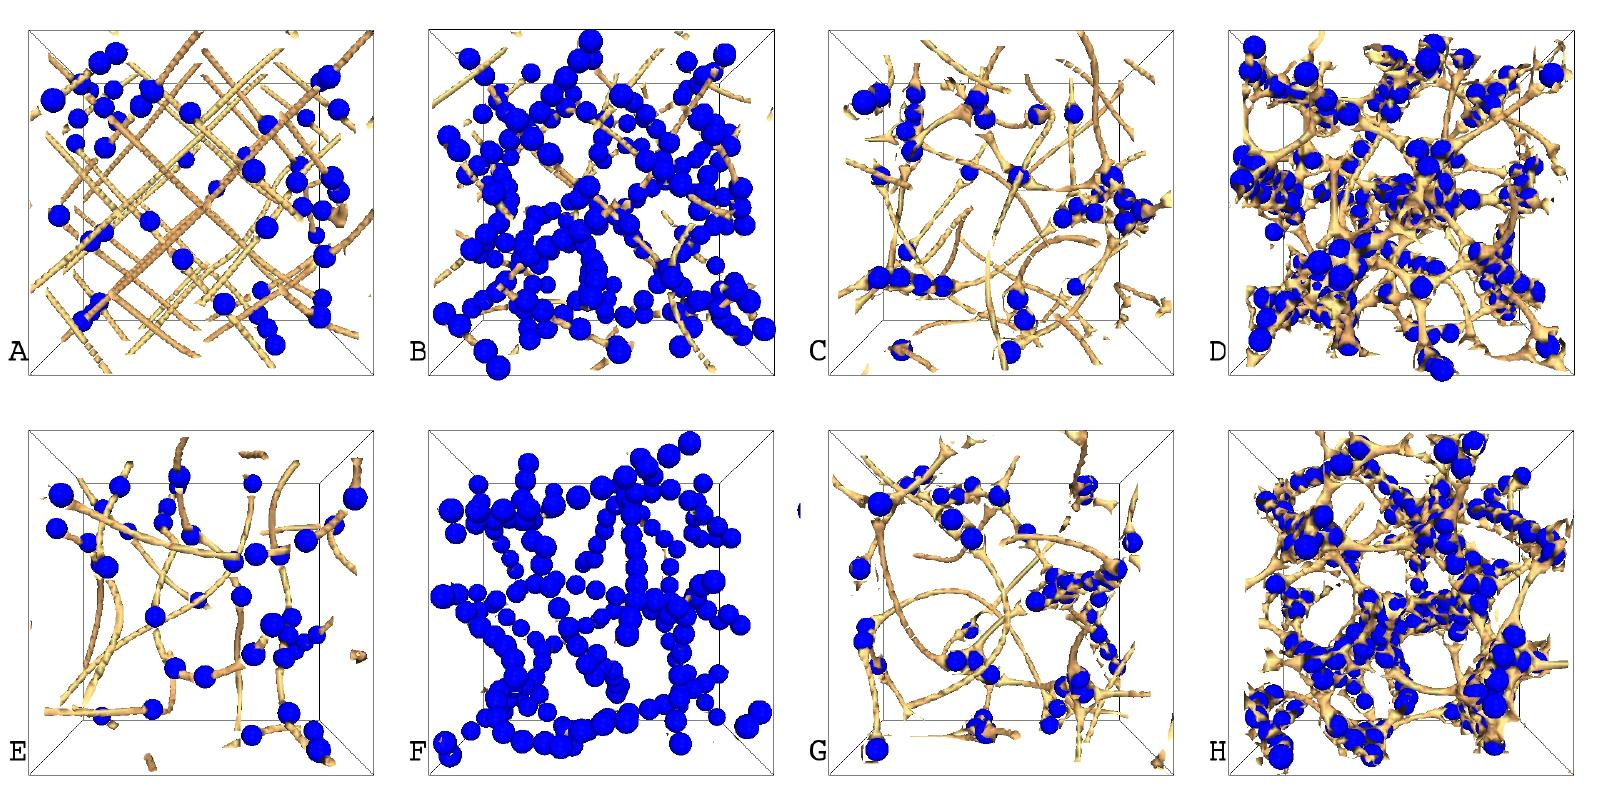
\includegraphics[width=\textwidth]{text-fig1.jpg}}
\caption{Snapshots of the states obtained after dispersing
a suspension of colloidal nanoparticles within a cholesteric liquid
crystal in the BPI-forming region. (A-D) correspond to the case
of a dispersion of particles in a pre-equilibrated BPI phase;
(E-H) are obtained by dispersing colloids in an isotropic
phase and then quenching into the range where BPI is stable, leading to formation of an amorphous, BPIII-like, disclination network.
Structures correspond
to (A,E) $w=0.23$ and $\phi=1\%$, 
(B,F) $w=0.23$ and $\phi=5\%$, 
(C,G) $w=2.3$ and $\phi=1\%$,
(D,H) $w=2.3$ and $\phi=5\%$.
The anchoring of the director field to the colloidal surface is normal.
[For the full parameter list used to generate Figs.~1-3 see Supporting Information.] For clarity, only a portion of the simulation box (a quarter of
each axis in size) is shown; the full structures are shown in Fig. S2 and S3.}
\end{figure}


\begin{figure}
\centerline{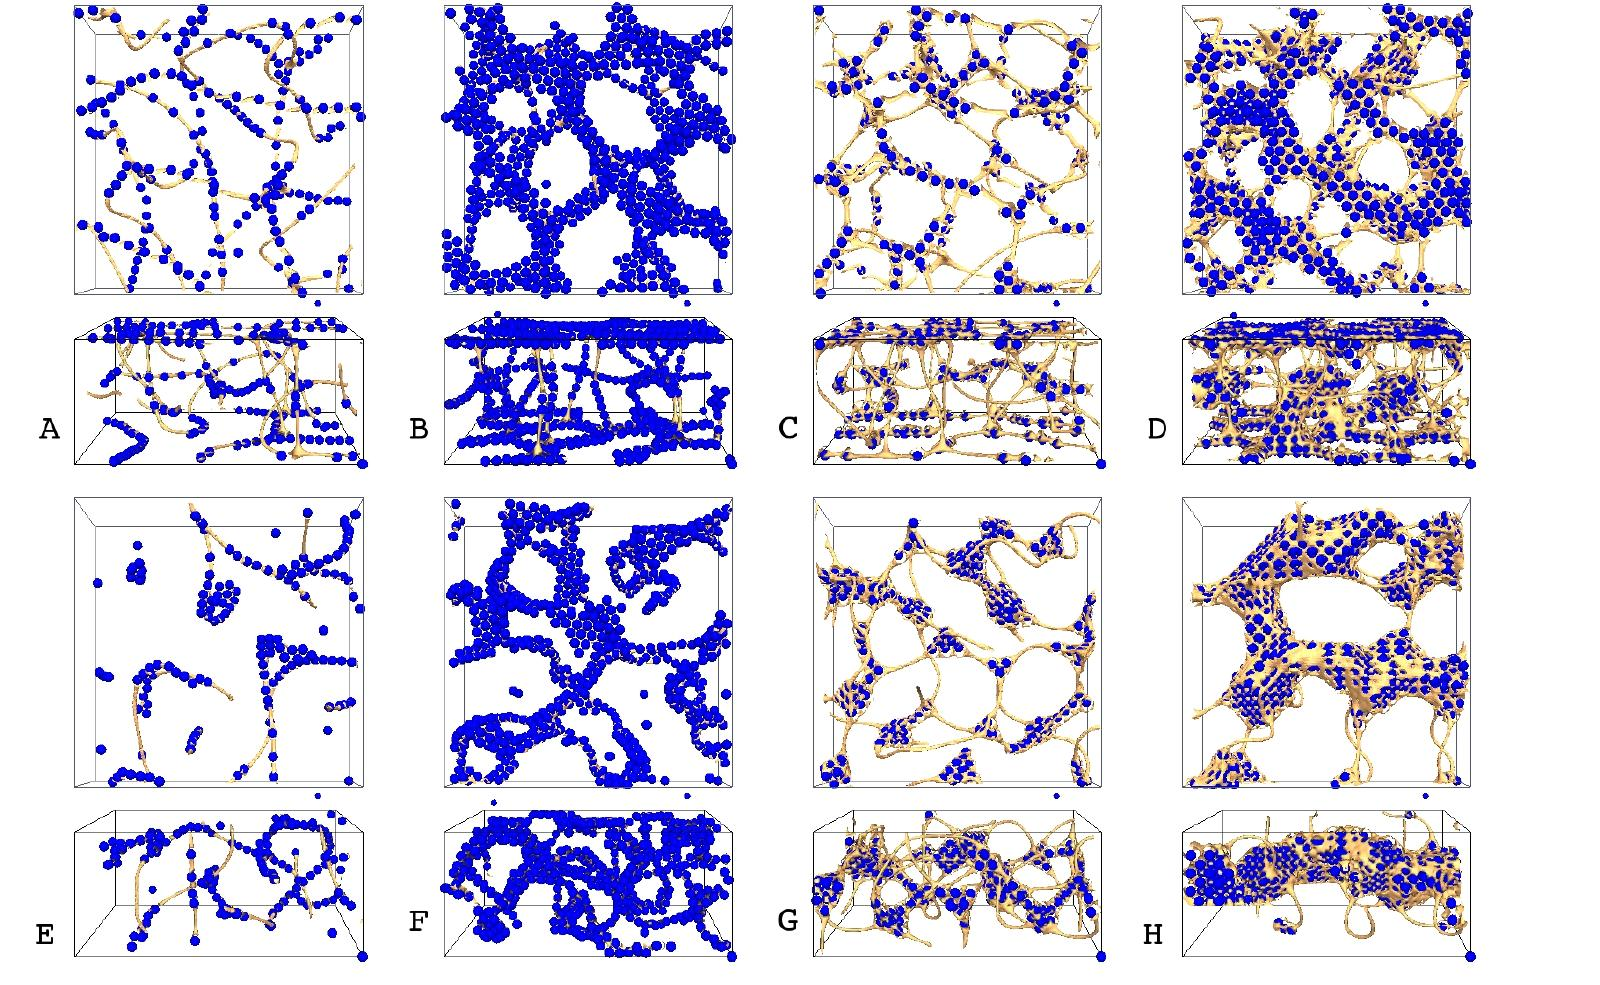
\includegraphics[width=\textwidth]{text-fig2.jpg}}
\caption{Snapshots of the steady states obtained when a dispersion of colloids in the isotropic phase is placed in a sandwich geometry, 
and then quenched into a regime where BPI is stable in the bulk. Both top and side views are provided.
The anchoring of the director field at the walls is normal for (A-D) and planar for (E-H). 
Structures correspond to (A,E) $w=0.23$ and $\phi=1\%$, 
(B,F) $w=0.23$ and $\phi=2\%$, 
(C,G) $w=2.3$ and $\phi=1\%$,
(D,H) $w=2.3$ and $\phi=2\%$.
As in Fig. 1, only a portion of the simulation box is shown for clarity;
the full structures are shown in Fig. S5 and S6.}
\end{figure}


\begin{figure}
\centerline{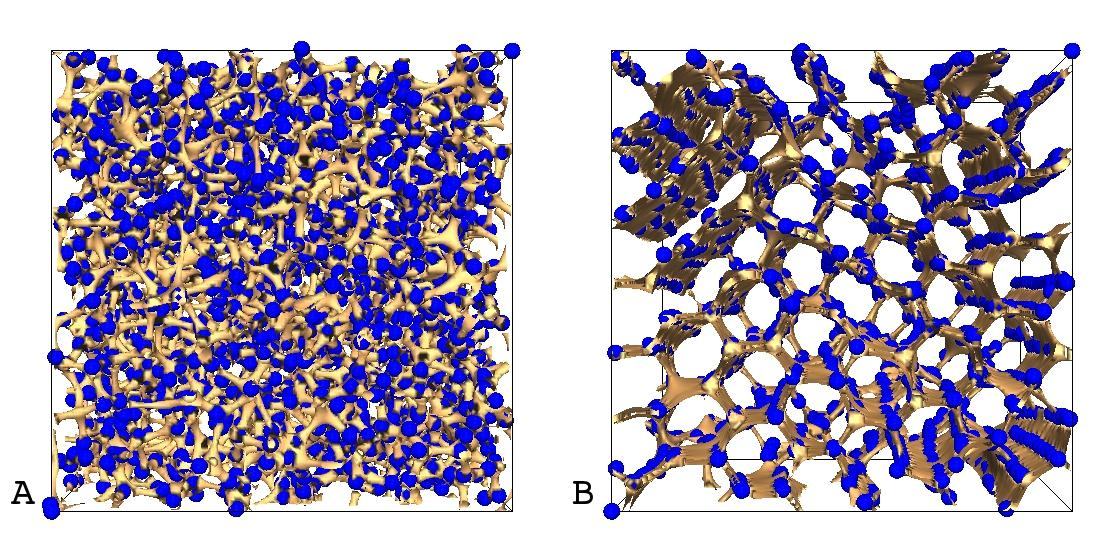
\includegraphics[width=\textwidth]{text-fig3.jpg}}
\caption{Snapshots of the steady states obtained when a dispersion of colloids is inserted into a thermodynamically stable bulk-BPIII (A), and finally subjected to an electric field along the vertical direction (B). The electric field leads to the formation of a honeycomb structure with hexagonal ordering perpendicular to the field direction. 
Structures correspond to $w=0.23$ and $\phi=1\%$ (see Supporting Information
for full list of parameters). }
\end{figure}

\end{document}
